\documentclass[spanish]{beamer}
\usepackage{babel}
\usepackage{marvosym} % \MVRIGHTarrow
% Theme choice:
\usetheme{Madrid}
\usecolortheme{} % beaver, seahorse

% Title page details: 
\title{Desobediencia Tecnológica y Software Libre}

\author{Iván Jijón}
\institute{ FLISoL 2023, Quito - Ecuador}
\date{\today}
\logo{      
    
\includegraphics[width=3.5cm]{img/flisol-banner-social.png}
}

\begin{document}

% Title page frame
\begin{frame}
    \titlepage
\end{frame}


% ToC frame
\begin{frame}{Contenido de la charla}
    \tableofcontents
\end{frame}

% Presentation structure
\section{Definiciones}
    \subsection{Tecnología}
    \subsection{Desobediencia}
\section{¿Qué es \bf{Desobediencia Tecnológica}?}
    \subsection{Estudio de caso: Cuba durante el Período Especial}
    \subsection{¿Qué \bf{dificultades} pretende \bf{resolver}?}
    \subsection{¿Cuál es su \bf{propuesta}?}
\section{En el mundo del Software}
    \subsection{¿Cuáles son las dificultades presentes en el \bf{Software Privativo}?}
    \subsection{Similitudes entre \bf{Desobediencia Tecnológica} y \bf{Software Libre}}
\section{Bibliografía y enlaces de interés}


\begin{frame}{Definiciones}
    \begin{block}{Tecnología - Oxford Languages}
        \begin{enumerate}
            \item Conjunto de los \emph{conocimientos} propios de una técnica.
            \item Conjunto de \emph{instrumentos, recursos técnicos o procedimientos} empleados en un determinado campo o sector.
        \end{enumerate}                             
    \end{block}
    \centering
    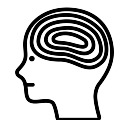
\includegraphics[width=3.5cm]{img/mind.jpg}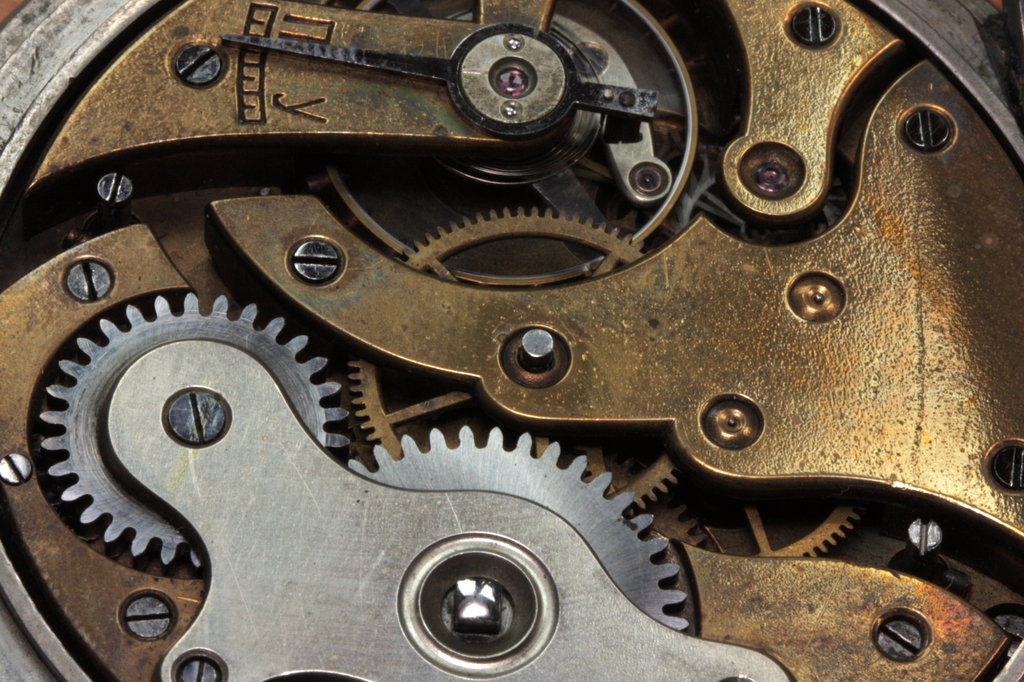
\includegraphics[width=3.5cm]{img/clockwork.jpg}
\end{frame}
\begin{frame}{Definiciones}
    \begin{block}{Desobediencia - Diccionario panhispánico del español jurídico, RAE}
        \begin{enumerate}
            \item Derecho penal: Rechazo activo u omisivo a dar cumplimiento a una orden vinculante y de exigible cumplimiento.
        \end{enumerate}
    \end{block}
    \begin{block}{Artículo 98 - Constitución de la República del Ecuador}
        Los individuos y los colectivos podrán ejercer el derecho a la resistencia frente a acciones u omisiones del poder público o de las personas naturales o jurídicas no estatales que vulneren o puedan vulnerar sus derechos constitucionales, y demandar el reconocimiento de nuevos derechos.
    \end{block}
\end{frame}
\begin{frame}{Definiciones}
    \begin{quote}
        "La desobediencia es el verdadero fundamento de la libertad. Los obedientes deben ser esclavos." ― H.D. Thoreau
    \end{quote}
\end{frame}

\begin{frame}{¿Qué es \bf{Desobediencia Tecnológica}?}
    \begin{block}{Desobediencia Tecnológica}
        Un conjunto de acciones creativas producto del cuestionamiento de los objetos y lógicas industriales.    
    \end{block}
    El término "Desobediencia Tecnológica" se publica por primera vez por Ernesto Oroza, artista y diseñador cubano en 2009.
    \vspace{0.3cm}
    
    \centering
        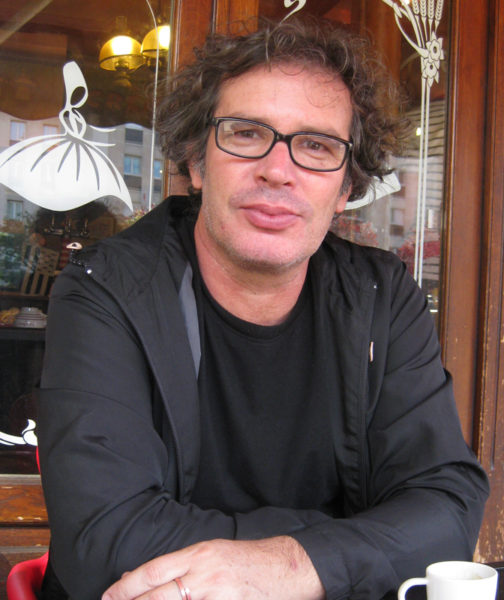
\includegraphics[height=4.5cm]{img/ernestooroza.jpg}
        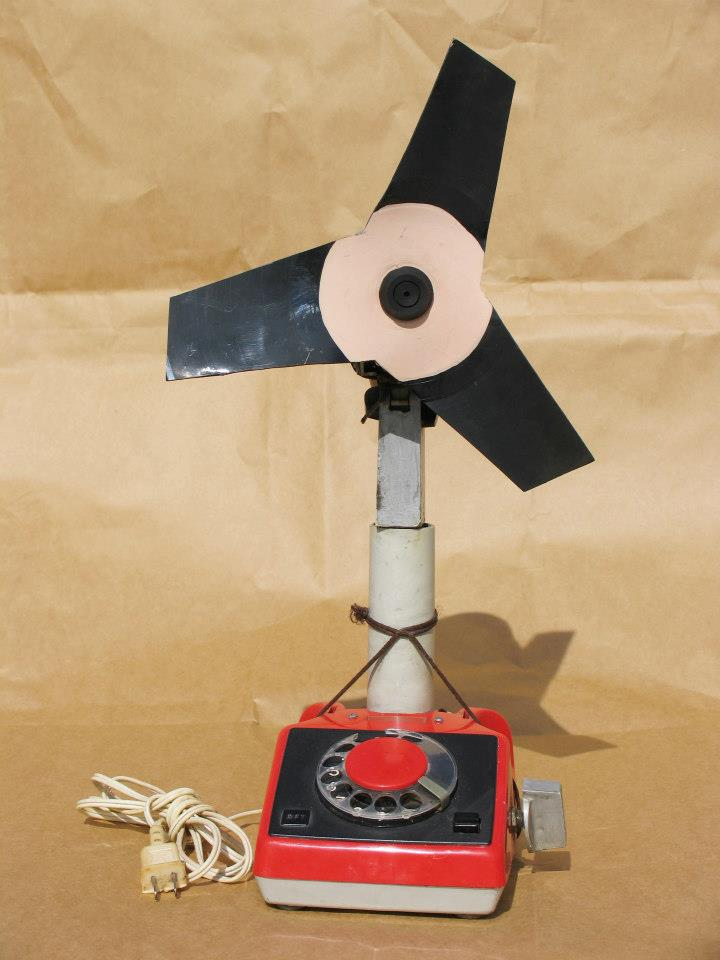
\includegraphics[height=4.5cm]{img/inventos/ventilador.jpg}
        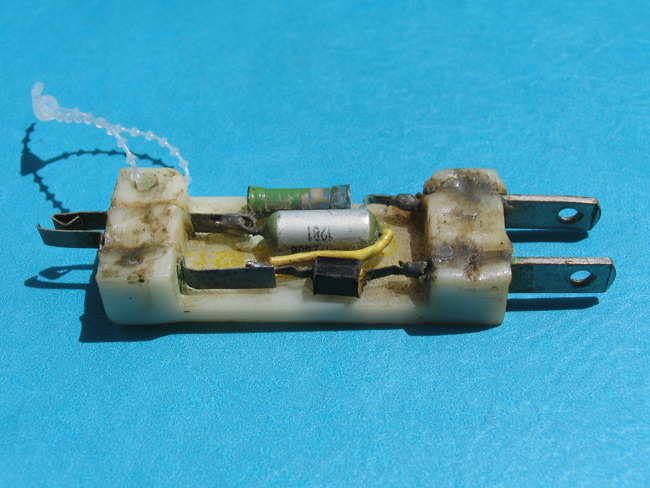
\includegraphics[height=3cm]{img/inventos/battery_charger.jpg}
        
\end{frame}

\begin{frame}{\bf{Desobediencia Tecnológica}: Contexto}   
    \begin{itemize}        
        \item 1991: caída de la Unión Soviética, economía cubana en implosión.
        \item Se intensifican las necesidades.
        \item El gobierno cubano incita a la gente a trabajar con máquinas: reparar, inventar para responder a la necesidad.        
    \end{itemize}
    \begin{center}            
        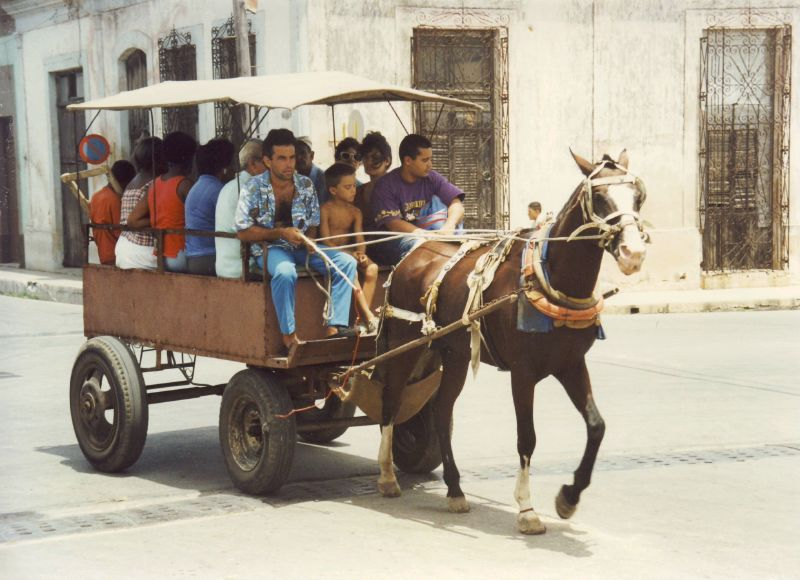
\includegraphics[height=4cm]{img/periodo_especial.jpg}
    \end{center}
\end{frame}

\begin{frame}{\bf{Desobediencia Tecnológica}: Limitaciones}      
    Dentro de las limitaciones que encontraron, algunas impuestas por el fabricante, están:
    
    \begin{itemize}
        \item el ciclo de vida de los objetos 
        \item el objeto industrial cerrado, hermético
        \item el diseño no incluye la posibilidad de reparar o de ser intervenido por el usuario
        \item la falta de un manual técnico, además del manual de uso
        \item la complejidad técnica        
    \end{itemize}    
\end{frame}

\begin{frame}{\bf{Desobediencia Tecnológica}: Comportamiento}        
    
    El ingenio se posiciona por encima del aparato.
    \vspace{0.3cm}
    \begin{columns}
        \column{0.25\linewidth}
            \centering
            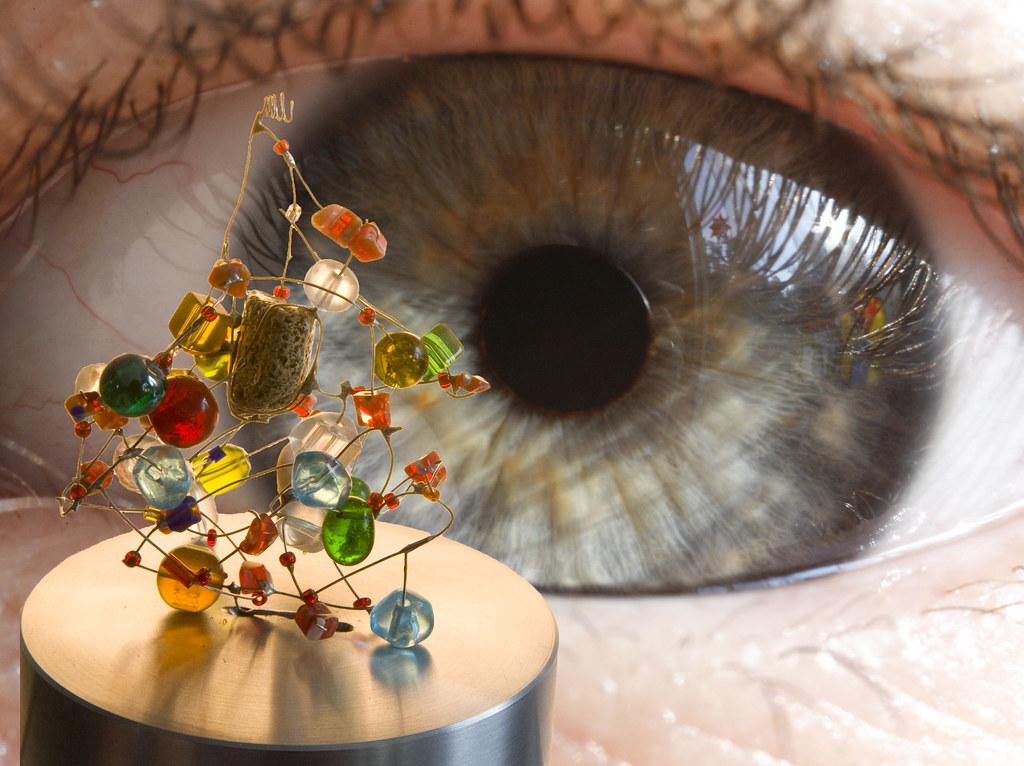
\includegraphics[width=3.5cm]{img/complejidad.jpg}
        \column{0.75\linewidth}
            \begin{itemize}
                \item Nueva mentalidad: ver el objeto por dentro, estudiarlo, entender cada componente.
                \item El aparato deja de ser una entidad única.
                \item Se aprende a reparar, reutilizar, modificar, crear.
            \end{itemize}
    \end{columns}
    \vspace{0.3cm}
    Esto permite saltar las barreras éticas, económicas, legales y estéticas impuestas por los fabricantes.
    Se logra una \emph{liberación moral}.
\end{frame}

\begin{frame}{\bf{Desobediencia Tecnológica}: Objetos de la necesidad}
    \begin{center}            
        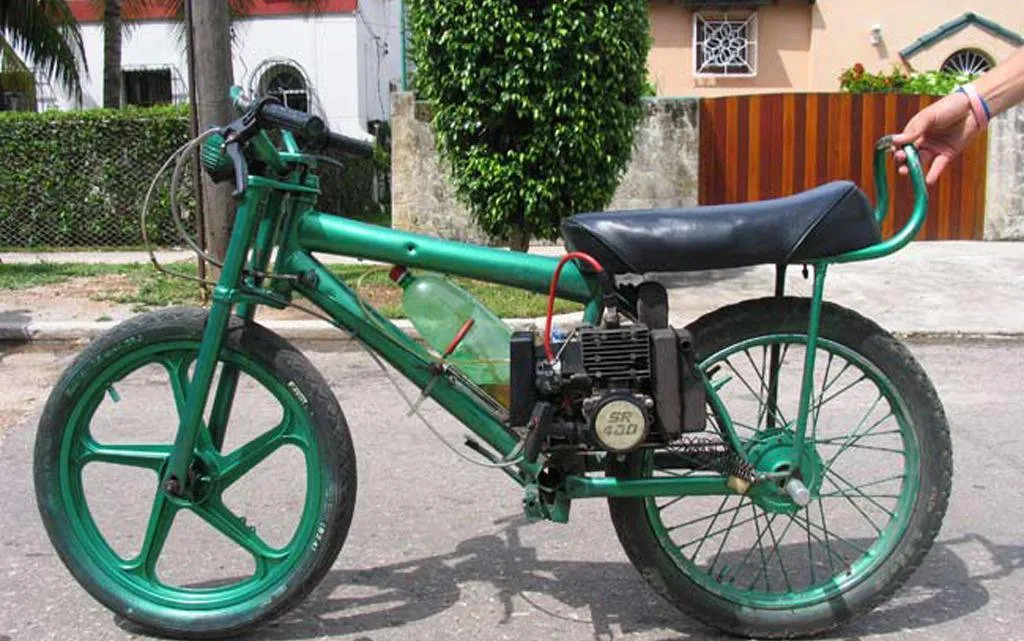
\includegraphics[height=3cm]{img/inventos/rikimbili.jpg}
        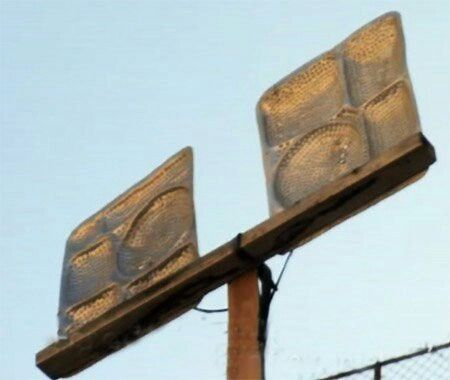
\includegraphics[height=3cm]{img/inventos/antena_bandejas.jpg}
    \end{center}
\end{frame}

\begin{frame}{Bibliografía y enlaces de interés}
    - Beamer para la presentación

    
\end{frame}

\end{document}